\documentclass{mnnit}
\usepackage{graphicx}
\usepackage{url}
\begin{document}

\title{Typing Test}
\author{Aaditya Supriyo\\Aakriti Gupta\\Abhishek Gupta\\Abhishek Kumar}\\ ~ \\ ~ \\~\\~\\~\\
\supervisor{Prof. M.M. Gore}
\specialization{Computer Science \& Engineering}
\beforepreface
\prefacesection{Preface}
A good wtyping test for any department in college is very usefull for the students to improve their typing speed. You can check your typing speed and accuracy online. Compare it with other results in the rankings and increase it using Ratatype. We measure your typing speed in WPM (words per minute). It is a calculation of how fast you type words with no typos. By the "word" we mean an average of 5 characters including spaces. We measure gross speed in our typing test. Typing Test that we made, using PHP, MySQL and Bootstrap, caters all of these requirements and helps the students to improve their typing skills.\\

\prefacesection{Acknowledgements}
Our Extreme gratitude to \textbf{Prof. M.M Gore} who guided us throughout the developement of \textbf{Computer Science And Engineering Department Web Portal}. Without his willing disposition, spirit of accomodation, timely clarification and above all faith in us, this project could not have been completed in due time.\\
We would also like to thank \textbf{Prof.A. K. Singh }, Head of the Department, Computer Science and Engineering Department (CSED), for providing us with all the needed resources and facilities during the process of completion of this project work.
Also we wish to gratefully acknowledge the assistance and cooperation, guidance provided by the staff of \textbf{Computer Science and Engineering Department(MNNIT)} during the development of this project. \\
Finally, we express our indebtedness to all who have directly or indirectly contributed to the successful completion of our report.
\afterpreface

\chapter{Introduction}

\section{Objective}
To create a Typing Test for the Computer Science and Engineering Department which will help students to increase their typing test as well as their accuracy.
\section{About The Project}
This is a advanced PHP,HTML,CSS,Bootstrap Typing Test system that will allow you to place a table and a few blocks of code on your website and get a detailed statistical information on your user's typing ability, including:
\begin{itemize}
    \item Words Per Minute (WPM)
    \item Accuracy Percentage Rating
    \item Total Words Typed
    \item Good Words / Bad Words Typed (Errors)
    \item Time Taken to Complete
    \item More as needed.
\end{itemize}

\section{Motivation}
As a student of Computer Science and Engineering Department, we have always felt the need for an online system that will improve our typing skills. During exam times,it becomes quite difficult to code with moderate typing skills hence, not being able to complete the entire exam.\\
From learning aspect, we wanted to work on a full web-app and apply all the concepts that we have learned in the past 2 years of our experience. We not only wanted to write the code, but also write Unit Tests for the same so that we can have some experience before we get into the industry.

\section{Related Work}
Since currently we do not have any Typing Test for CSED, we had to look for other sources for related work. \textbf{Online website-Typing Master}\cite{Refworks=1} is a frequentry used website for conducting typing tests which gave us some of the insight to the final product and the set of features that we are planning to achieve.

\chapter{Design Methodology Used}
We used the basic Waterfall Model to Develop our project.\\
In waterfall model we follow the following steps to develop the project
\begin{enumerate}
\item Gather and document requirements
\item Design
\item Implement
\item Perform testing
\item Maintenance
\end{enumerate}
This model is very simple to understand and implement. However, due to its\\
simplicity, this model is only useful for a limited type of projects.\\\\
Following are the reasons why we chose this model:
\begin{enumerate}
\item Our requirements were rigidly defined from the very beginning.
\item The technology that we were going to use was very well defined.
\item Each phase of the project was clearly defined.
\end{enumerate}


\chapter{Proposed Work}
The system that we are planning to build should support the following basic functionality:
\begin{itemize}
  \item Typing Test for students.
  \item Platform for improving typing skills for individuals.
  \item Results will be displayed after taking the test.
  \item Details of all the students taking the test.
  \item Selection of any language.
\end{itemize}

\section{Advantages of proposed work}
\begin{itemize}
    \item The students will be able to take the test anytime anywhere.
    \item Students will become more efficient and can thereby enhance their skills.
    \item Students can easily register for the test and view their results as well.\\~\\
    
\end{itemize}

\section{Functional and Non-Functional Requirements}
\subsection{Functional Requirements}
The Typing Test must support the following features:
\begin{itemize}
    \item The admin should be able to add or remove students appearibg for the test.
    \item The web-app should be responsive to support portable devices like mobile phones.
    \item The system must log every admin login.
    \item The system should provide security against basic attacks like SQL Injection and XSS.
\end{itemize}
\subsection{Non-Functional Requirements}
\begin{itemize}
    \item The web-app should be designed in such a way that it should be easy for others to maintain and add new features.
    \item The UI/UX of the web-app should be intuitive as well as visually appealing.
    \item The web-app should support web page caching to reduce the response time.
    \item All the functionality of the web-site should be easily testable using automated Unit Tests.
\end{itemize}
\chapter{Software/Hardware Requirements}
\subsection{Software Requirements}
\begin{itemize}
    \item PHP 7.0
    \item xDebug: Used to generate test coverage reports for Unit Tests.
    \item MySQL: RDBMS of our choice, though we can easily use some other SQL based DBMS.
    \item Apache HTTP Server
\end{itemize}
\subsection{System Requirements}
\begin{itemize}
    \item Intel Core (or Dual Core 2GHz) or equal AMD CPU.
    \item 2GB RAM or Above
    \item 40GB of Free HDD Space
\end{itemize}

\chapter{Design}
\section{ER Diagram}
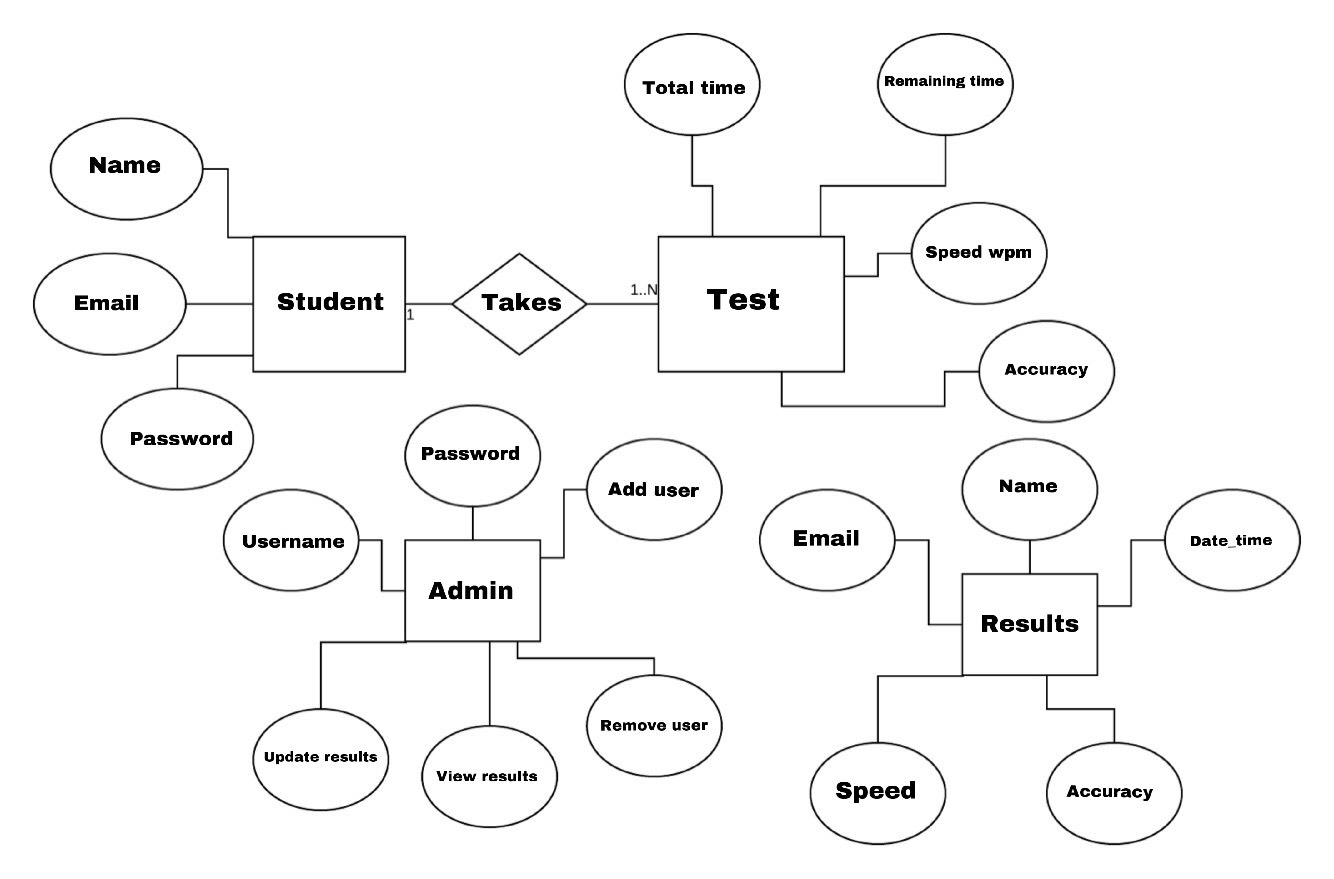
\includegraphics[width=\textwidth, height=350pt]{images/ER.jpg}
\chapter{Implementation}
\section{Architectural Pattern}
For implementation, \textbf{Model-View-Controller (MVC)} architectural pattern that is an industry standard for Web Apps. In this we have divided the project into three modules:
\begin{itemize}
    \item \textbf{Model}: The model is the central component of the pattern. It is the application's dynamic data structure, independent of the user interface.
    \item \textbf{View}: A view can be any output representation of information, in this case, they represent the HTML pages that we show the users.
    \item \textbf{Controller}: Acts as a interface between the Model and View.
\end{itemize}

\section{PHP Framework}
To make the project more scalable and easier for future users to modify, we wanted to use a framework. Instead of defining one of our own, which will make it difficult for the future users to understand the code, we decided to choose one of the following best possible PHP Frameworks that support MVC available in the market.
\begin{itemize}
    \item \textbf{Laravel}
    \item \textbf{Codeigniter}
\end{itemize}
Since the footprint of Codeigniter was smaller than that of Laravel, we went ahead with the same. Though Laravel supports more features, those features also make it more complex\cite{Refworks=4}. Also one of the disadvantages of Codeigniter when compared with Laravel was its below average integration with PHPUnit which we solved by using \textbf{ci-phpunit-test for CodeIgniter 3.x}.\cite{Refworks=5}
\section{Naming Convention}
Before we actually started the implementation, we decided on some of the naming convention that we will use throughout the project. Following are the list of those:
\begin{itemize}
    \item \textbf{PHP}: PHP do not have a common naming standard that can be followed, so we decided to use the one that the official Codeigniter website recommends.\cite{Refworks=2}
    \item \textbf{MySQL}: We followed the naming convention from sqlstyle.guide to be followed throughout the project.\cite{Refworks=3}
\end{itemize}
\section{Module Details}
\subsection{Model}
This module deals with all the database interactions for the application. It acts as an intermediate gateway for Controller to access the database. Following are classes are a part of this module:
\begin{itemize}
    \item \textbf{Model\_admin:} interacts with \textbf{admin} table. Currently supports just one operation i.e. manage\_user.
    \item \textbf{Model\_event:} interacts with \textbf{event} table and performs operations on it.
    \item \textbf{Model\_login:} enables the student to login and store it's details in the database.
    \item \textbf{Model\_signup:} fetched the deatils from the database to authorize the student details.
    \item \textbf{Model\_typing:} enables the student to take up the test.
    \item \textbf{Model\_result:} allows the student to view their results after taking the test.
\end{itemize}
\subsection{Controller}
This module acts as an interface between database and view. 
\begin{itemize}
    \item \textbf{Admin:} interacts with \textbf{Model\_admin}
    \item \textbf{Event:} interacts with \textbf{Model\_event} and fetches the details of events.
    \item \textbf{Home:} interacts with \textbf{Model\_event} and \textbf{Model\_result} to load their results.
    \item \textbf{Typing:} interacts with \textbf{Model\_typing} and allows student to take the test. 
    \item \textbf{Student\_corner:} loads page with static information.
\end{itemize}
\subsection{View}
View module contains all the files that are responsible for generating the HTML code and receives its inputs from the controller. Each controller file is bounded with a view file where the corresponding controller queries from the model and sends the result to the input.\\
Some of the more elegant things about our implementation of view are
\begin{itemize}
    \item \textbf{Nav Menu:} To make the modification of Menu easier, the items in the menu are defined in the \textbf{menu\_items.json} file and are read by \textbf{menu.php} which inturn converts it into HTML code.
    \item \textbf{Default Template:} All the pages on the website include the same \textbf{header.php} and \textbf{footer.php}. Hence instead of including these files in every page, we have created \textbf{default.php} that includes both of these files and also loads the content of the page in between them.
\end{itemize}

\chapter{Testing}
\section{Unit Tests}
We have performed Unit Tests using PHPUnit which is a Unit Testing framework for PHP. Currently we have completed the test cases for \textbf{Model Module} with total line coverage of 85.83\%. Since Model accesses the Database, we have mocked all the calls to the database while testing and only testing the flow in the functions of those models.\\
We are also working on the test cases for \textbf{Controller Module} which has around 10\% code coverage as of now. Test cases for rest of the modules will not be needed since they will be covered once we finish up the test case for \textbf{Controller Module}\\\\
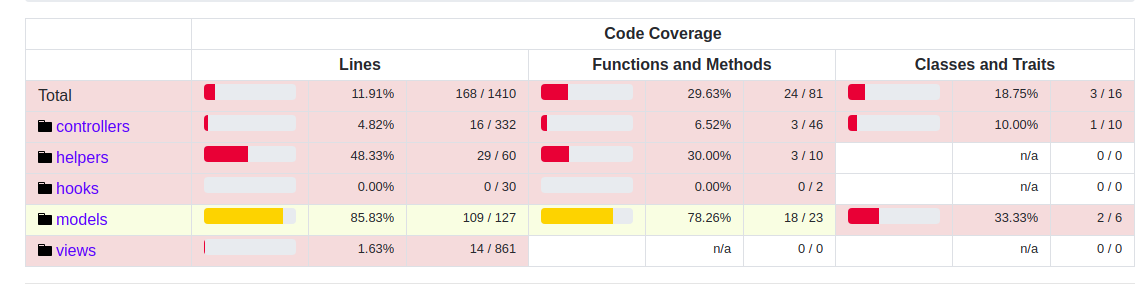
\includegraphics[width=\textwidth]{images/coverage.png}
\begin{center}
\emph{Code Coverage of Test Cases}
\end{center}
\section{Functional Tests}
Since not everything gets covered in Unit Tests, we performed manual functional tests to make sure that the basic functionalities do not have any bug.\\
Some of the features that we have tested are:
\begin{itemize}
    \item Accessing all the information on the site (Tests, Students, Results and more).
    \item Adding/Deleting Student Information.
    \item Adding/Deleting Tests and checking if the results are displayed properly.
    \item Adding/Deleting Test details.
    \item Adding/Deleting Languages or content of the test.
    \item Viewing all the Web-App on Multiple size windows so that we are sure its completely responsive.
    \item Trying to access modification rights without Admin Access.
\end{itemize}


\chapter{Screenshots}
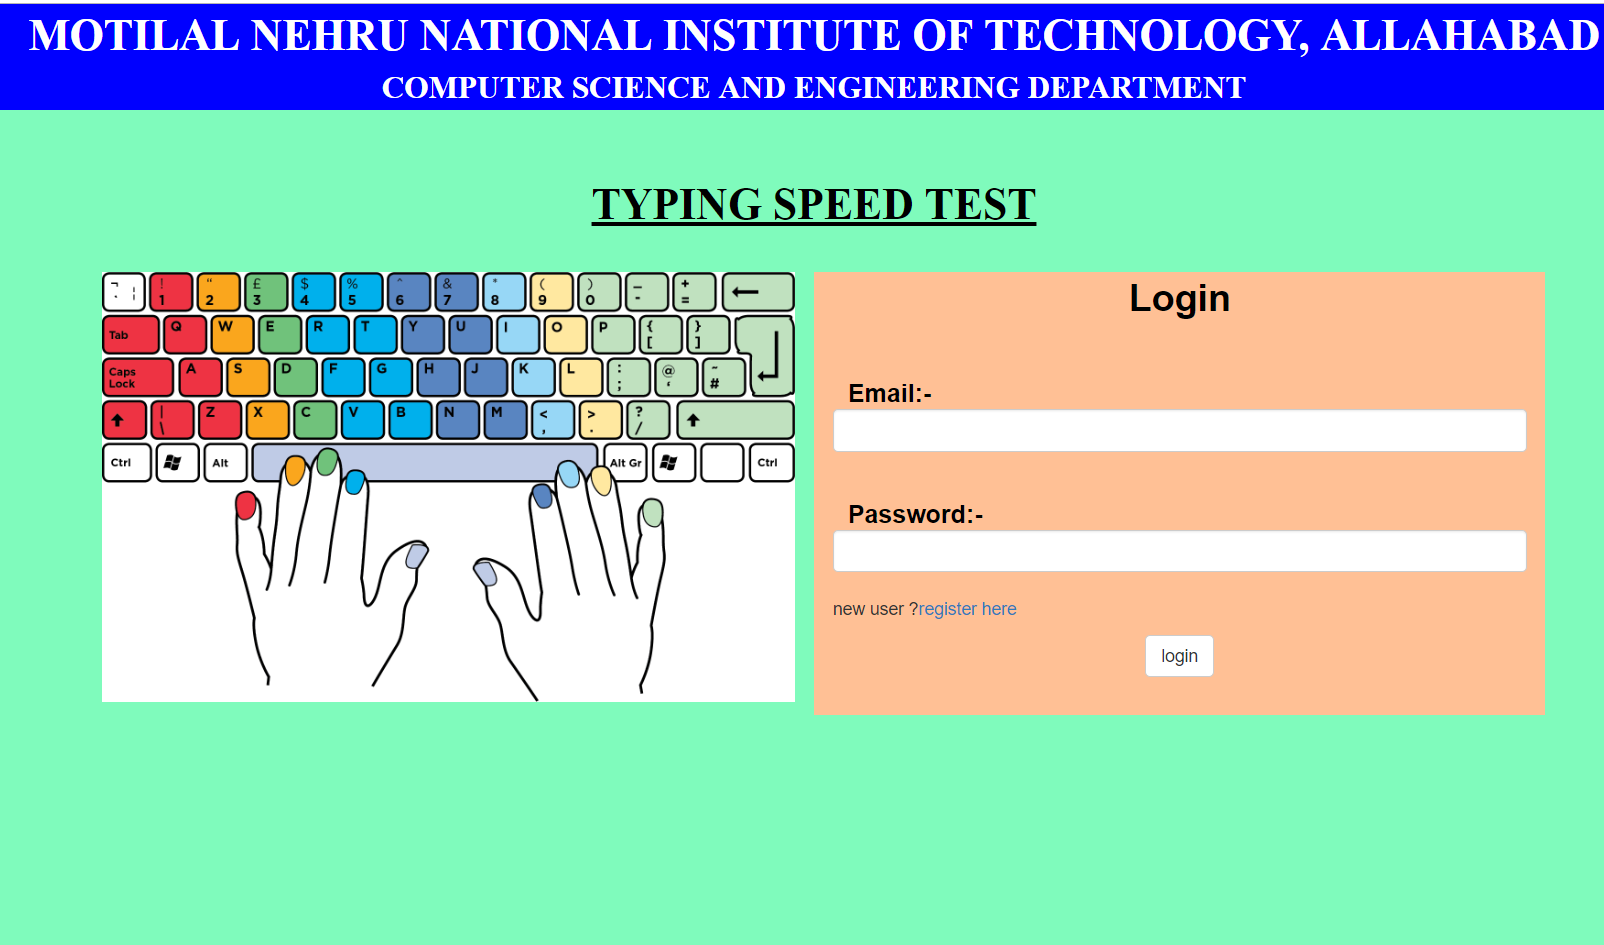
\includegraphics[width=\textwidth]{images/1_userLogin.PNG}
\begin{center}
Fig 5.1: \emph{Login page of portal}
\end{center}
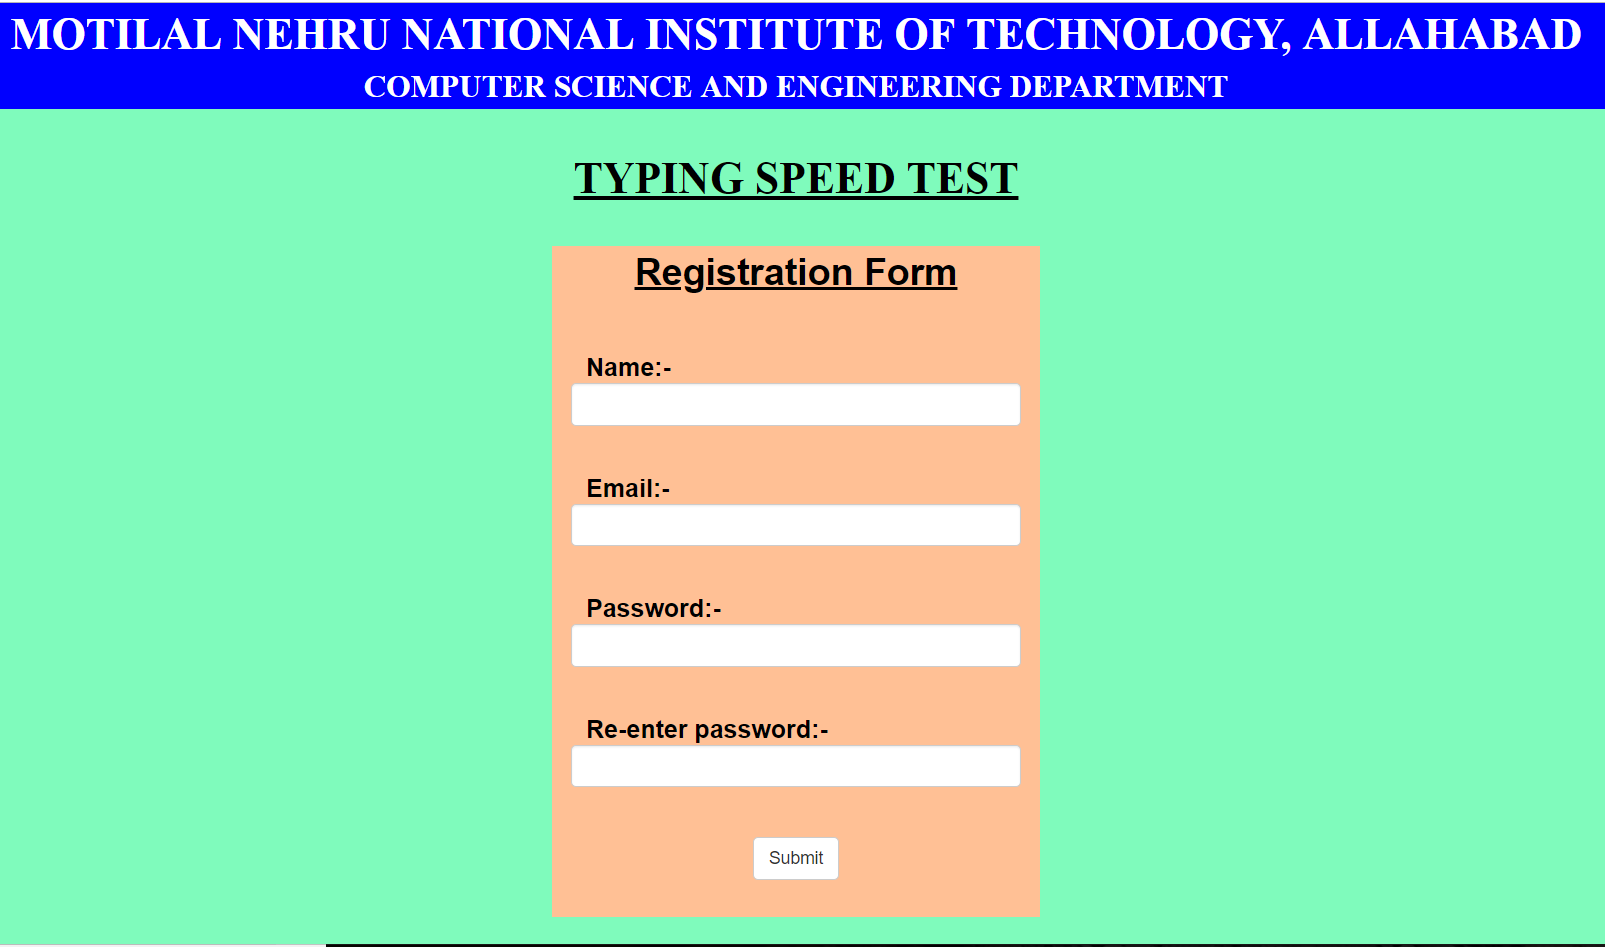
\includegraphics[width=\textwidth]{images/2_sinup.PNG}
\begin{center}
Fig 5.2: \emph{Faculty page: Signup page: Allows the user to register}
\end{center}
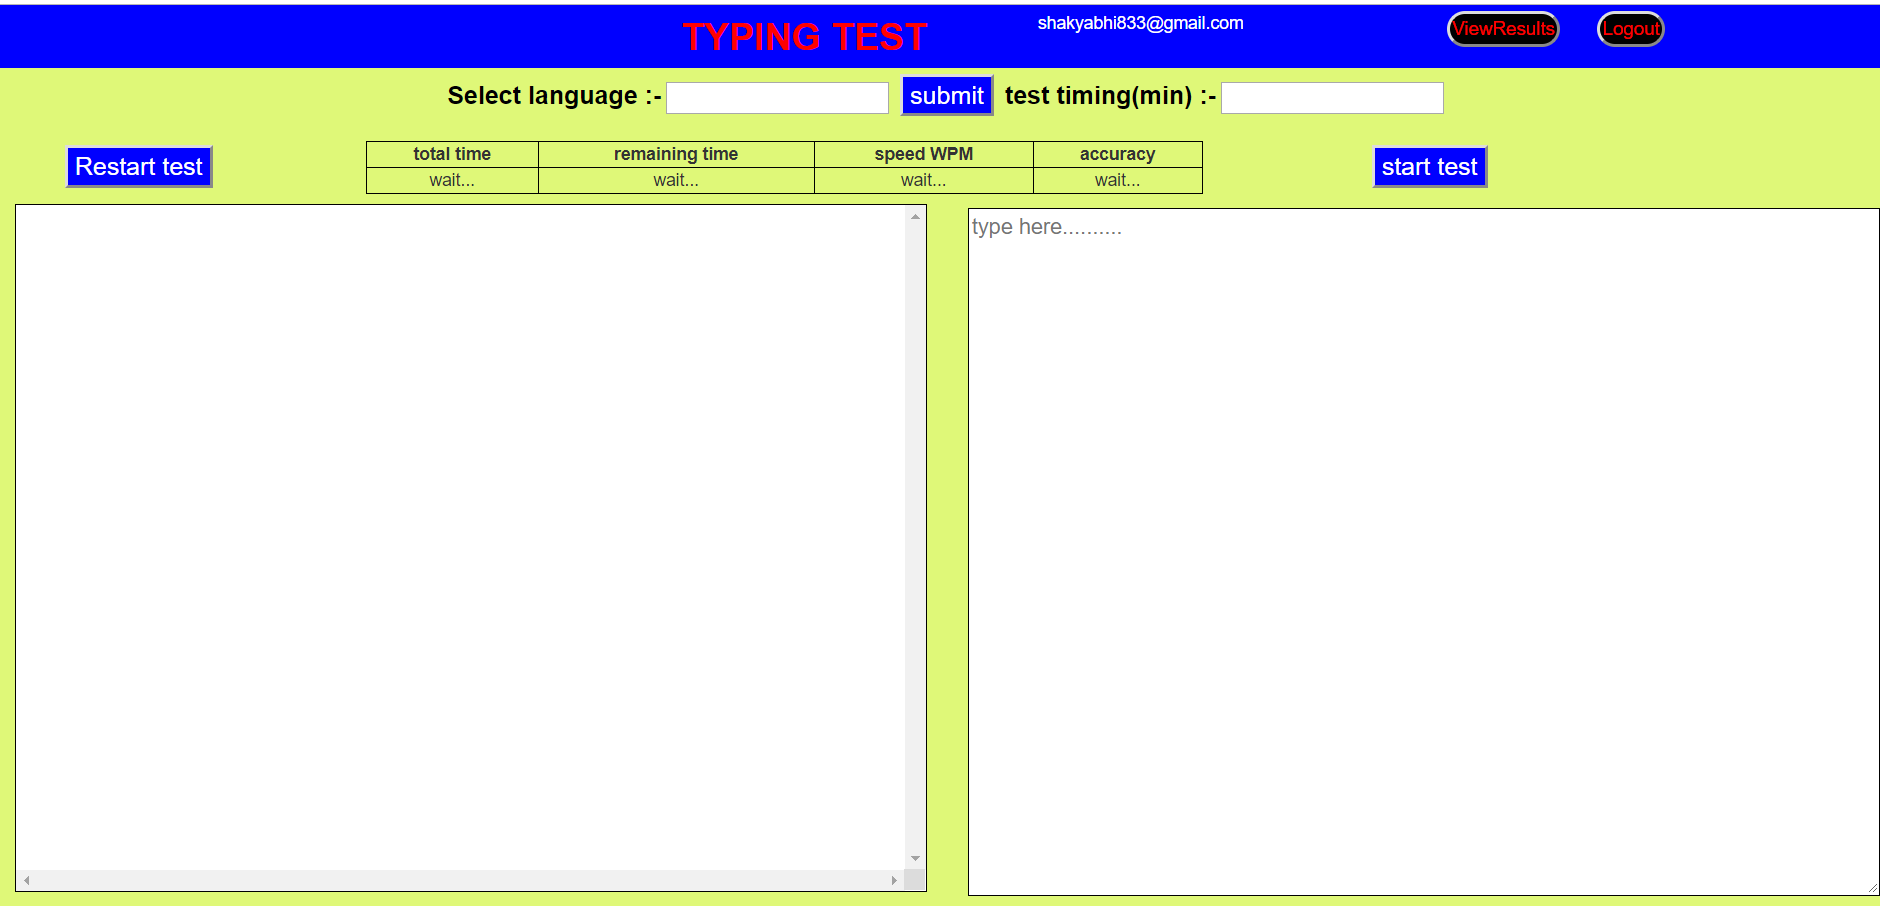
\includegraphics[width=\textwidth]{images/3_afterlogin.PNG}
\begin{center}
Fig 5.3: \emph{Test Page}
\end{center}
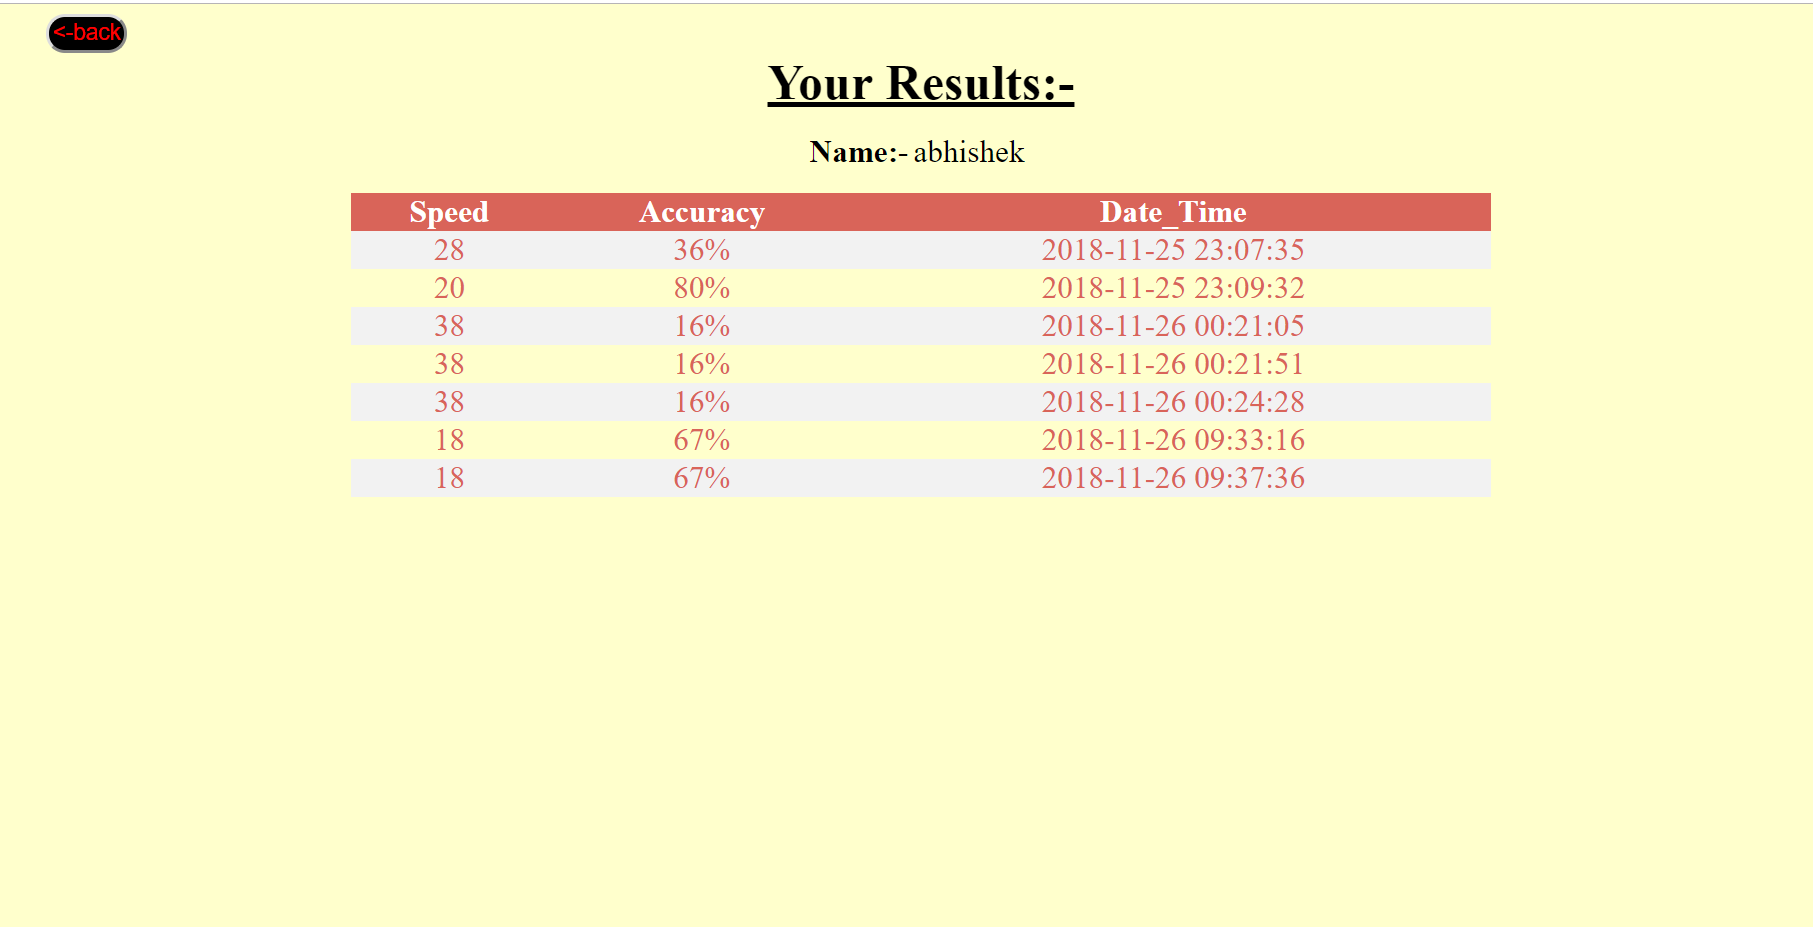
\includegraphics[width=\textwidth]{images/4_viewResultuser.PNG}
\begin{center}
Fig 5.4: \emph{Result: Display student's result.}
\end{center}
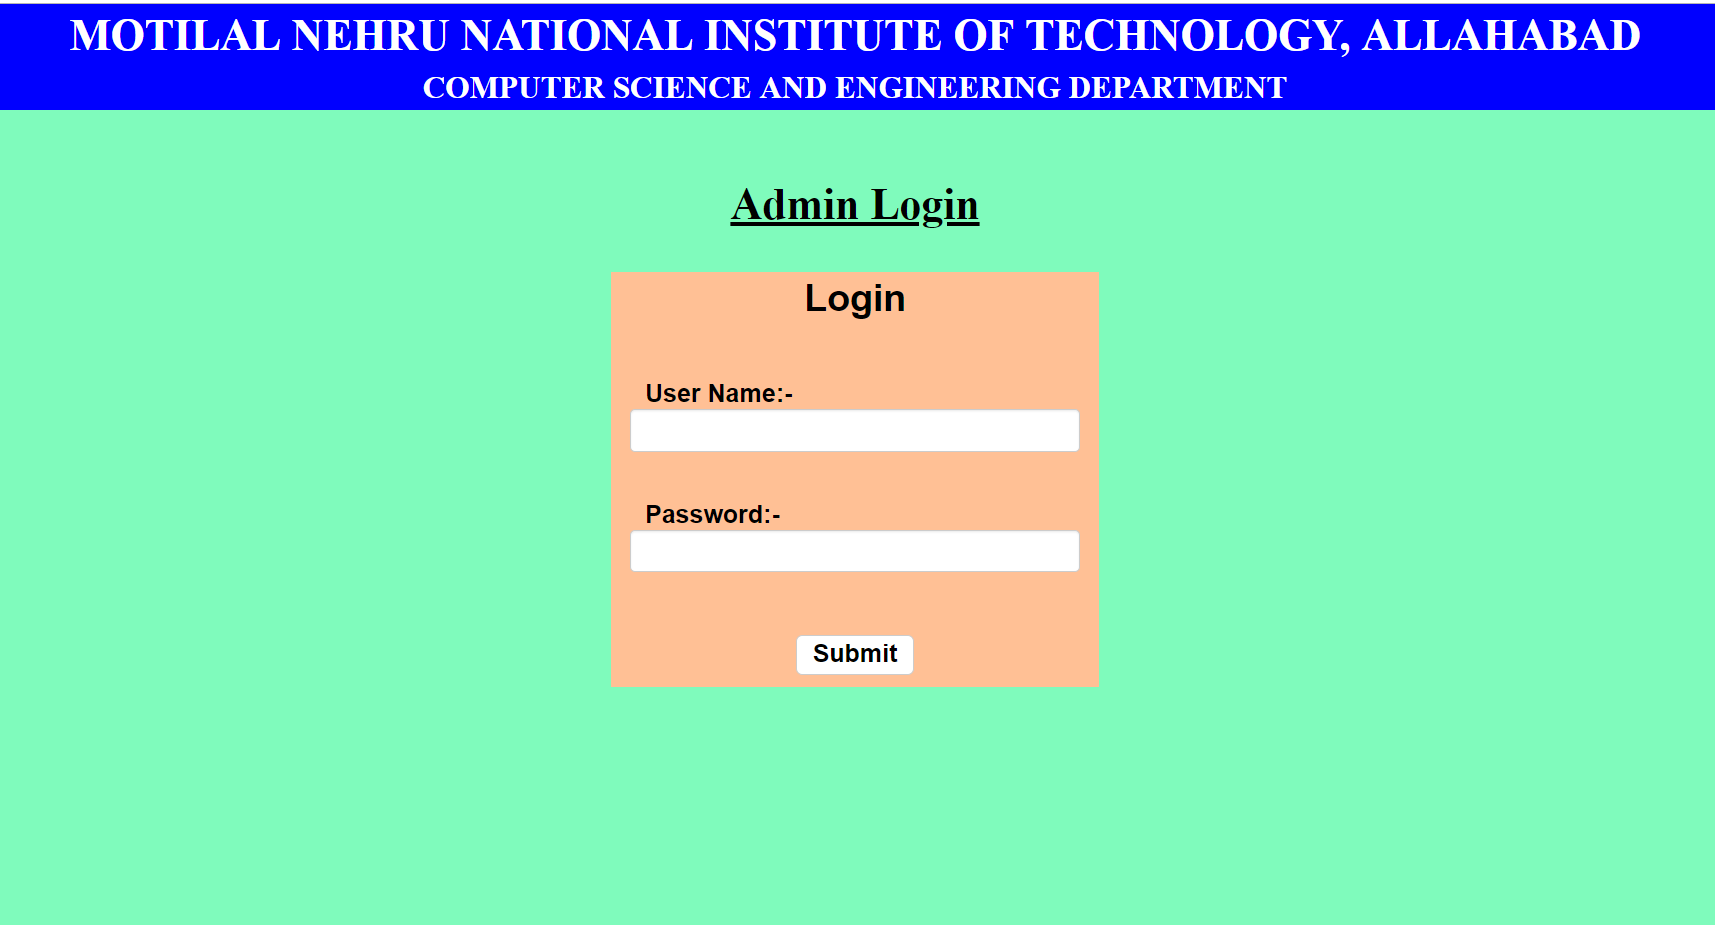
\includegraphics[width=\textwidth]{images/5_adminLogin.PNG}
\begin{center}
Fig 5.5: \emph{Allows Admin to login}
\end{center}
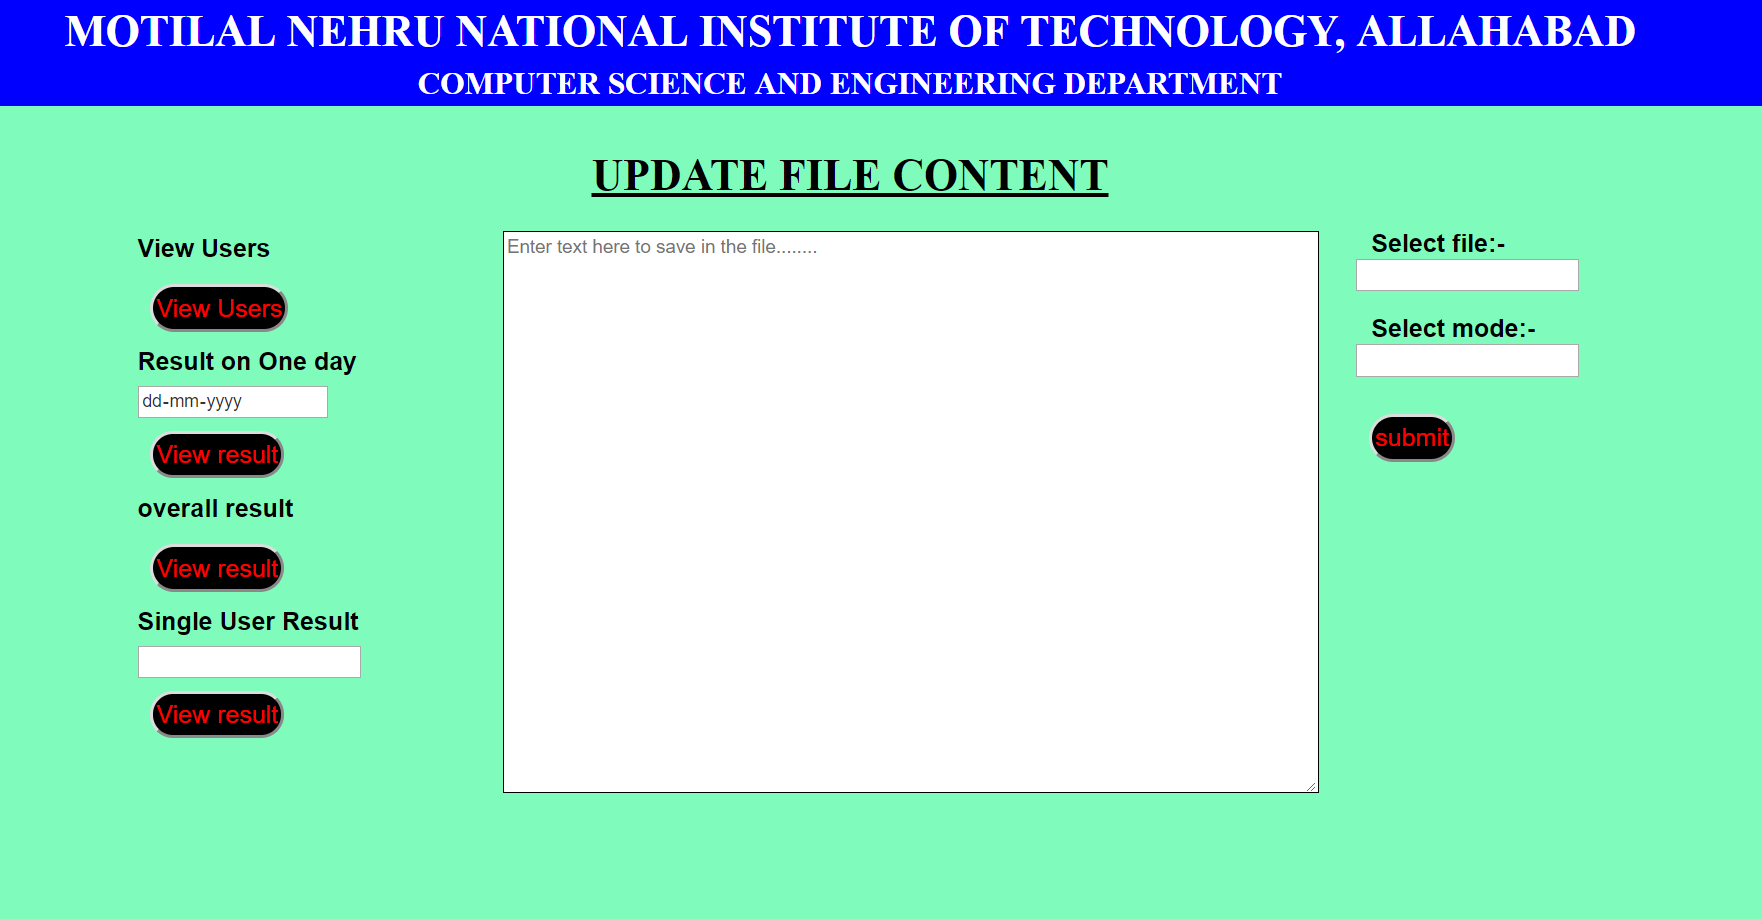
\includegraphics[width=\textwidth]{images/6_admindashboard.PNG}
\begin{center}
Fig 5.6: \emph{Admin Dashboard}
\end{center}
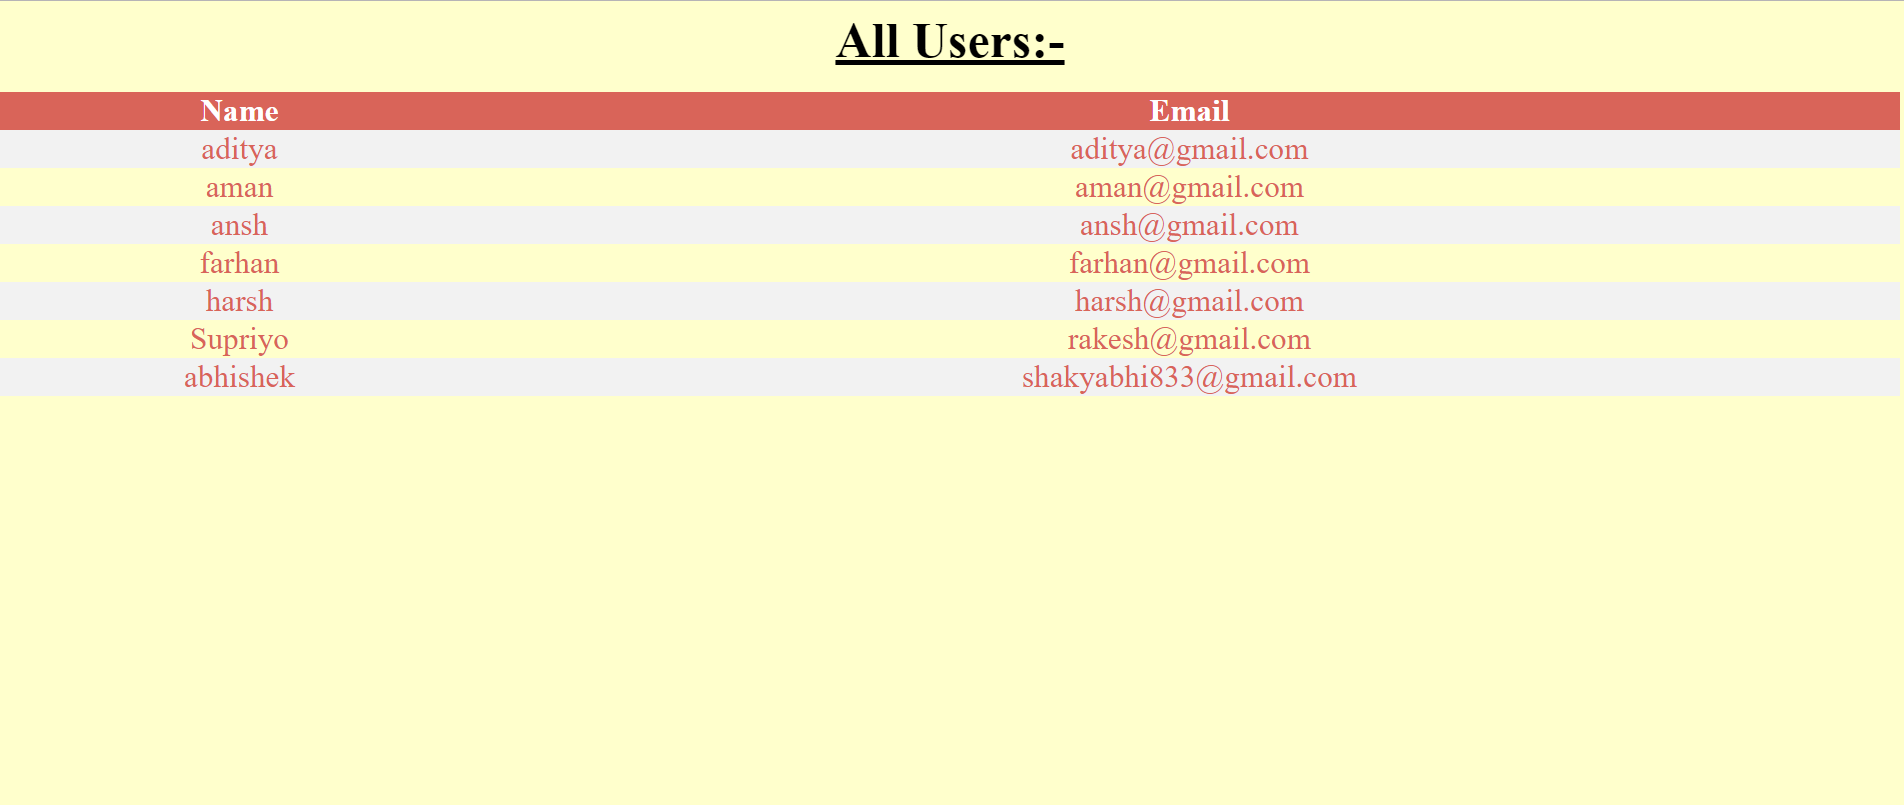
\includegraphics[width=\textwidth]{images/7_admin_view_allusers.PNG}
\begin{center}
Fig 5.7: \emph{Registered user page with Admin logged in}\\
\end{center}
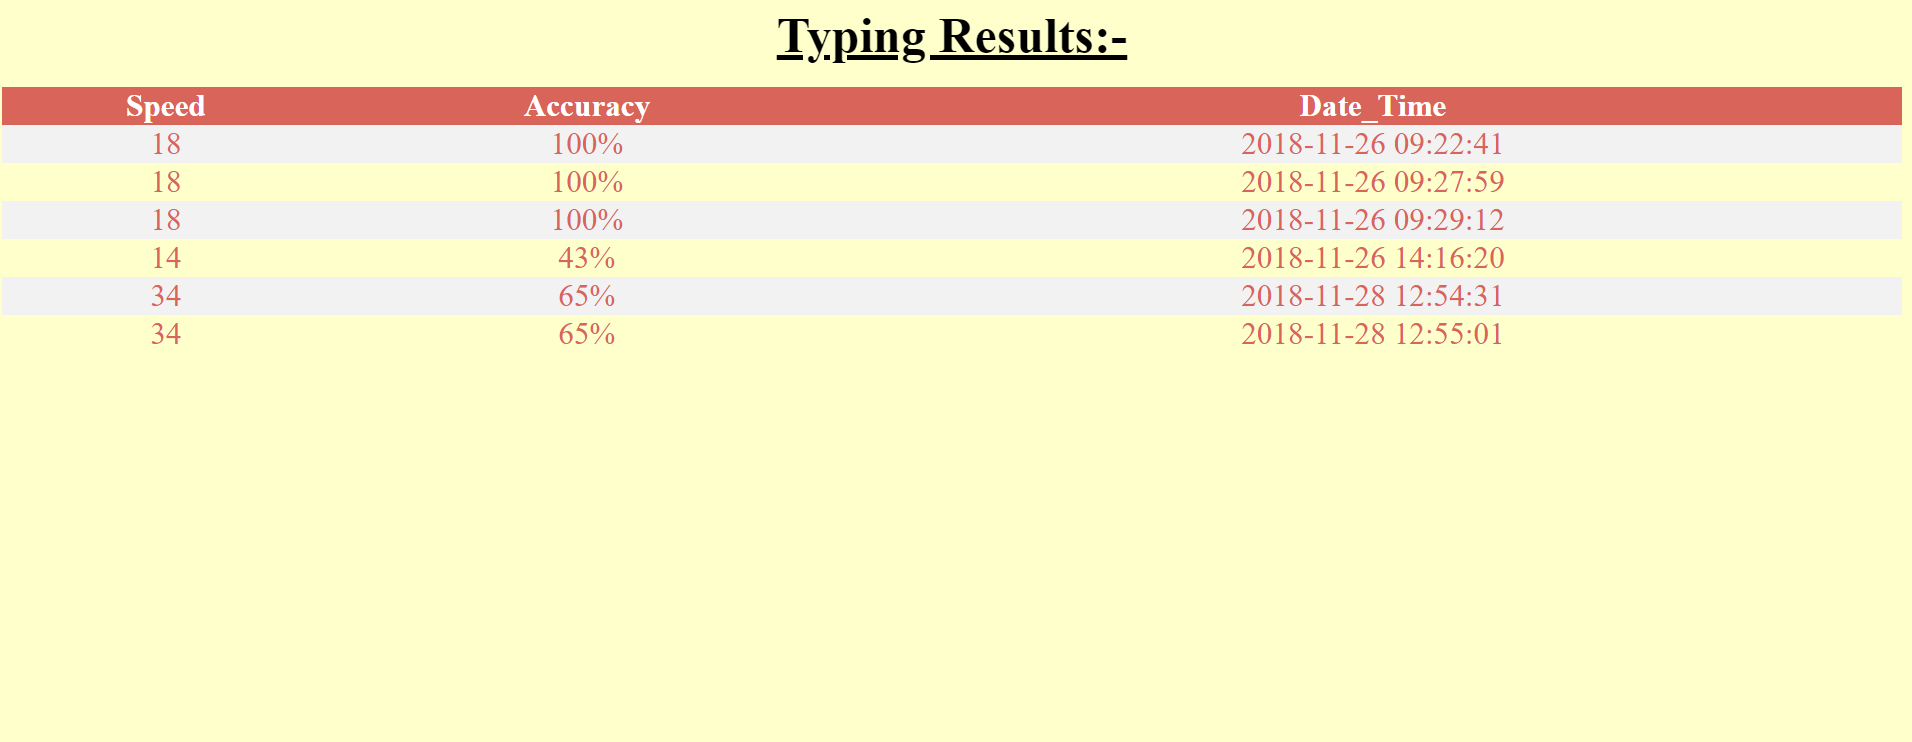
\includegraphics[width=\textwidth]{images/8_img.PNG}
\begin{center}
Fig 5.8: \emph{Admin can view Particular user result}\\
\end{center}
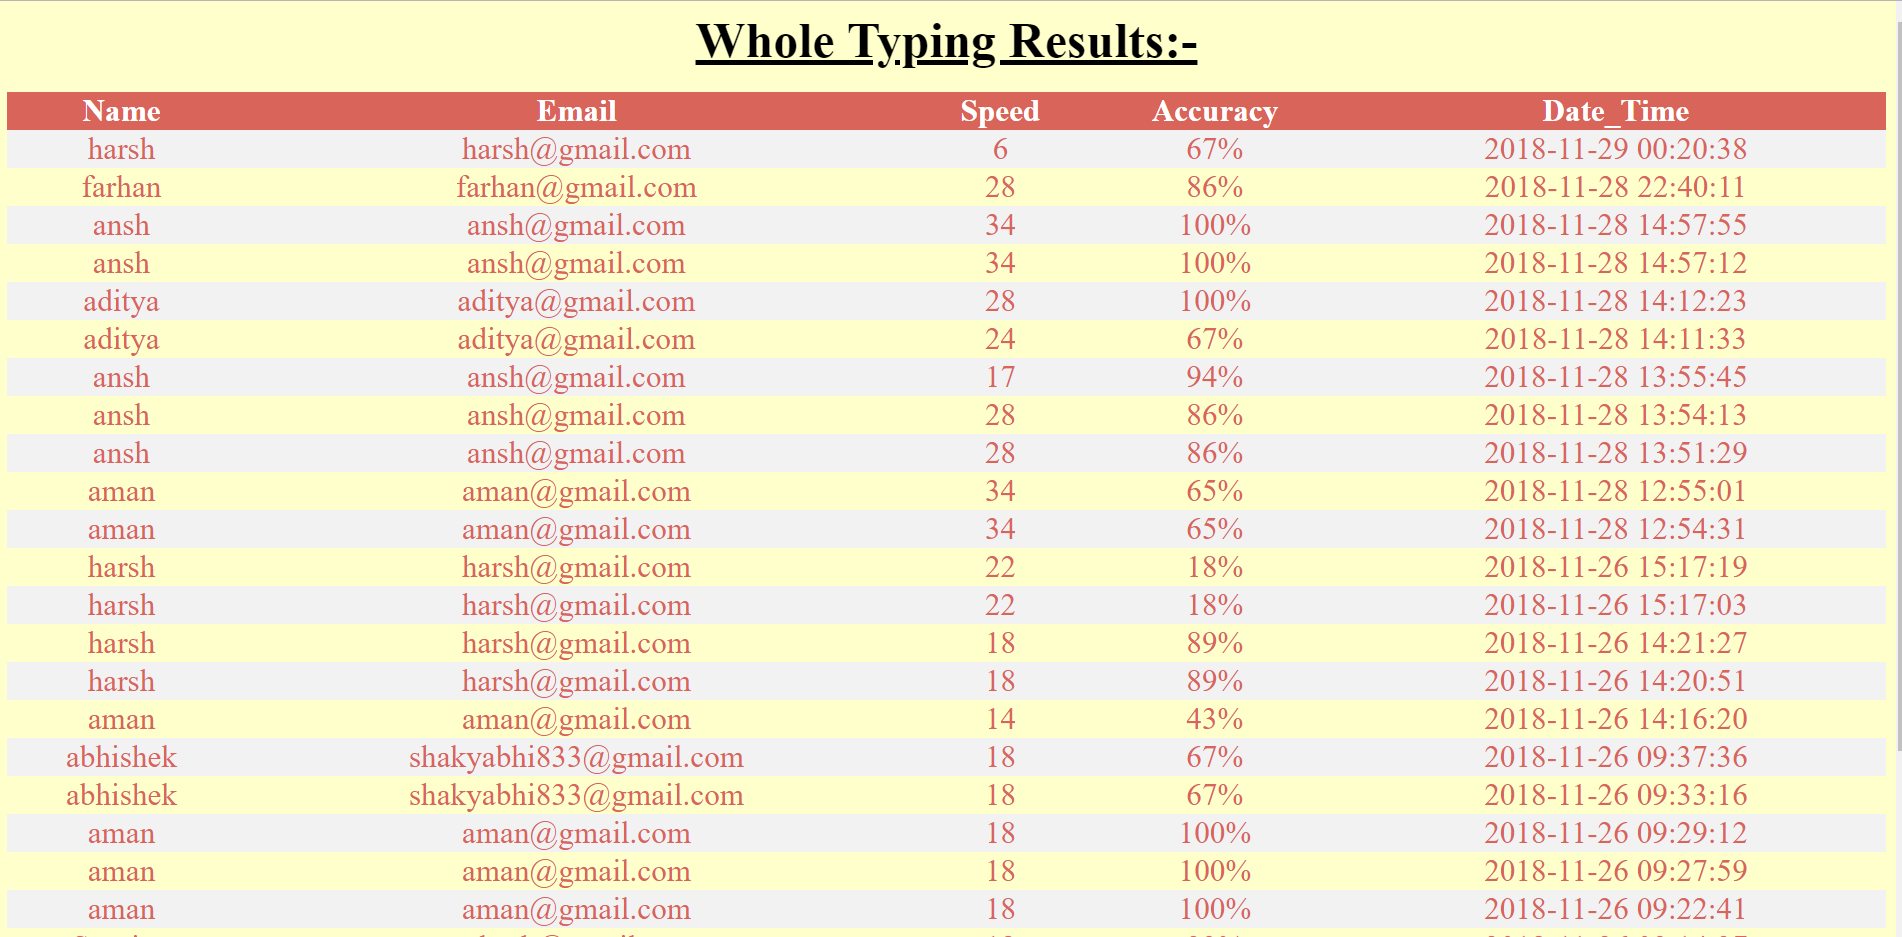
\includegraphics[width=\textwidth]{images/9_img.PNG}
\begin{center}
Fig 5.9: \emph{Admin can view all the typing results}\\
\end{center}
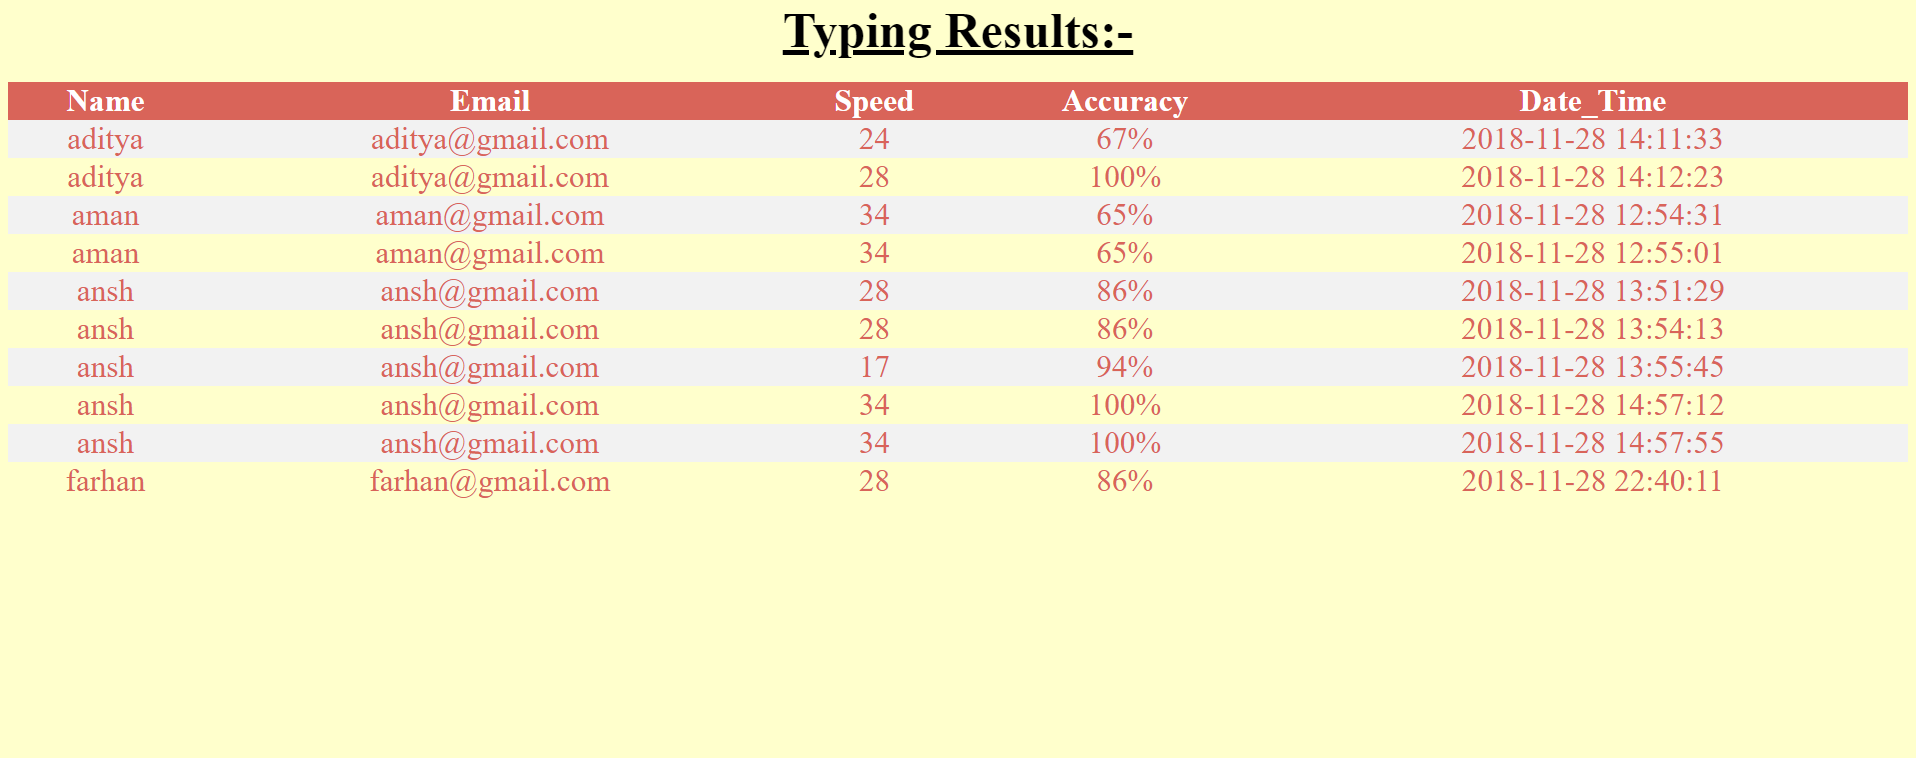
\includegraphics[width=\textwidth]{images/10_img.PNG}
\begin{center}
Fig 5.9: \emph{Admin can view results for particular date}\\
\end{center}
\user
\chapter{Conclusion and Future Work}
We now have a Web-app for our CSED Department that will be useful for the students to take the typing test anywhere from the campus to improve their skills. Though it may have a very limited number of features as of now, it can very easily be modified to add new features.\\\\
In future many other functionalities can be added to the portal like\cite{Refworks=1249}:
\begin{itemize}
    \item Adding sensor to check that right keys are pressed or not.
    \item Email notifications of results to students.
    \item Capture the picture of the student appearing for the test.
    \item Digital certificate will be generated after test result and can also be printed.
\end{itemize}



\bibliographystyle{acm}

\bibliography{references}

%\addcontentsline{toc}{chapter}{References}
\end{document}
